\subsection{The Disordered Ising Model}
The model under scrutiny in this article is the \emph{disordered Ising Ferromagnet}
which is derived from the well understood \emph{square lattice Ising Ferromagnet} \cite{Onsager1944}.
That is a square lattice with lateral length \(L\) and \(N=L^2\)
sites with periodic boundary conditions.
Each site has an Ising spin \(s \in \{-1,+1\}\) and interacts with its
nearest neighbors described by the Hamiltonian
\begin{equation}
    \mathcal{H} = - \sum_{\avg{i,j}}J_{ij}s_{i}s_{j}.
    \label{eq:hamiltonian}
\end{equation}
\(\avg{i,j}\) refers to nodes \(i\) and \(j\) which are nearest
neighbors, so that they are directly coupled to each other.
This will be called an edge.
The coupling between \(i\) and \(j\) is characterized by \(J_{ij} = J\),
the coupling constant.

The most important difference of the square lattice Ising model to the
disordered Ising Ferromagnet is that the sites of the square lattice are
displaced introducing geometric disorder resulting in a non regular graph
structure.
The displacement is randomly Gaussian distributed with standard
deviation \(\sigma\), i.e.\ the \(x\) and \(y\) coordinates of the
sites are displaced by random \(\Delta x\) and \(\Delta y\) drawn
from a Gaussian distribution
\begin{equation}
    f(\Delta x)=\frac{1}{\sqrt{2\pi}\sigma}\mathrm{e}^{-\frac{\Delta x^2}{2\sigma^2}}.
    \label{eq:gauss}
\end{equation}
This is sketched in Fig.\ \ref{fig:displacement}.
\begin{figure}[htbp]
    \centering
    \includegraphics[width=0.45\textwidth]{images/Displacement}
    \caption[Sketch how the Displacement works]
    {
        Sketch how the displacement of the nodes works. The nodes
        get displaced by \(\Delta x\) and \(\Delta y\) drawn from the
        distributions displayed next to the points. The original
        square lattice is indicated by dashed lines.
    }
    \label{fig:displacement}
\end{figure}
In the following \(\sigma\) will also be called \emph{disorder parameter}.
If we take "nearest neighbor" in the Euclidean meaning, most sites
will only have one nearest neighbor after the
displacement. If only the edges between these neighbors remained,
the lattice would collapse to many very small clusters. But if one
left the edges as they were before the displacement, the edges would
cross -- at least for big displacements. The crossing of edges then
would destroy the planar character of the model.
To avoid this, a new edge set will be etablished after the displacement.
The edges are constructed
so that for a given configuration of points the resulting graph is an
instance of a so called proximity graph. The coupling constant \(J_{ij}\) gets
identified with edge weights. \(J_{ij}\) will be changed to depend on the
geometric distance between the connected pair of sites. More precise,
the weight of an edge is
\begin{equation}
    E_{ij} = J_{ij} = \mathrm{e}^{(\alpha (1-d_{ij}))}
    \label{eq:coupling}
\end{equation}
where \(d_{ij}\) is the Euclidean
distance between the nodes \(i\) and \(j\). Following Ref.\ \cite{Lima2000}
the free parameter \(\alpha\) is set to \(\alpha = 0.5\).
The boundary is periodic, i.e.\ nodes near the right edge can be
connected to nodes near the left edge and vice versa. Analogously the
top and bottom edges are connected as if the graph lives on a torus.
In subsequent graphics the graphs will be unwrapped to rectangular
shapes. Connections which cross a periodic boundary are indicated
by edges which connect a solid node to a dashed node.
Note that for \(\sigma = 0\) all \(d_{ij} = 1\) and therefore all
\(J_{ij} = 1\), so that the disordered Ising model is reduced to the
square lattice Ising model.

\subsection{Proximity Graphs}
\label{ssec:graphtypes}
    A graph \(G(V,E)\) is a set of nodes \(V\) and edges \(E \subset V^{2}\).
    In the scope of this model, the nodes get identified with the sites of the
    lattice. If two nodes are connected by an edge, the sites are neighbors.\\
    All here mentioned graph types are \emph{proximity graphs}.
    The edges of these graphs connect nodes which are by some metric near
    to each other.
    Hence they are suited to generalize problems defined on regular
    lattices with nearest neighbor relationships.
    To determine the distance we use the Euclidean
    metric on two-dimensional graphs, though in principle every metric in any
    dimension can be used.\\

    \subsubsection{Gabriel Graph}
        The Gabriel graph (GG) \cite{Gabriel1969}
        is a subgraph of the Delaunay triangulation (DT) (for a definition
        see e.g.\ Ref.\ \cite{Katajainen}), i.e.\ for the same set of nodes
        \(V\) the edge set of the DT is a superset of the edge set of the
        GG \(E_{DT} \supseteq E_{GG}\). Two nodes \(i\) and \(j\) with distance
        \(d_{ij}\) will be connected with an edge, if a circle with its
        center on half way between \(i\) and \(j\) and radius
        \(r = \frac d 2\) contains no other nodes. This area will be
        called \emph{lune} in the following. See also the cross hatched region
        from Fig.\ \ref{fig:lunes}\subref{sfig:lunes:def}. An Example is
        given in Fig.\ ref{fig:lunes}\subref{sfig:lunes:gg}.

    \subsubsection{Relative Neighborhood Graph}
        The Relative Neighborhood
        graph (RNG) \cite{Toussaint1980} is a subgraph of the GG. Two nodes \(i\) and \(j\) with
        distance \(d_{ij}\) will be connected again, if no other node is in the
        \emph{lune}, which is different from the lune of the GG. The lune
        is defined as the intersection of two
        circles with radius \(r = d\) and centers on \(i\) and \(j\).
        See also the hatched region in Fig.\ \ref{fig:lunes}. An Example is
        given in Fig.\ ref{fig:lunes}\subref{sfig:lunes:rng}.

    \begin{figure}[htbp]
        \centering
        \subfigure[Definition of the Lunes][]{
            \label{sfig:lunes:def}
            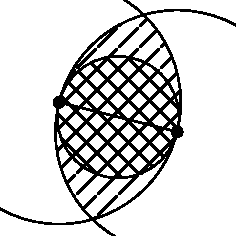
\includegraphics[width=0.14\textwidth]{images/GG_RNG_def}
        }
        \subfigure[RNG example][]{
            \label{sfig:lunes:rng}
            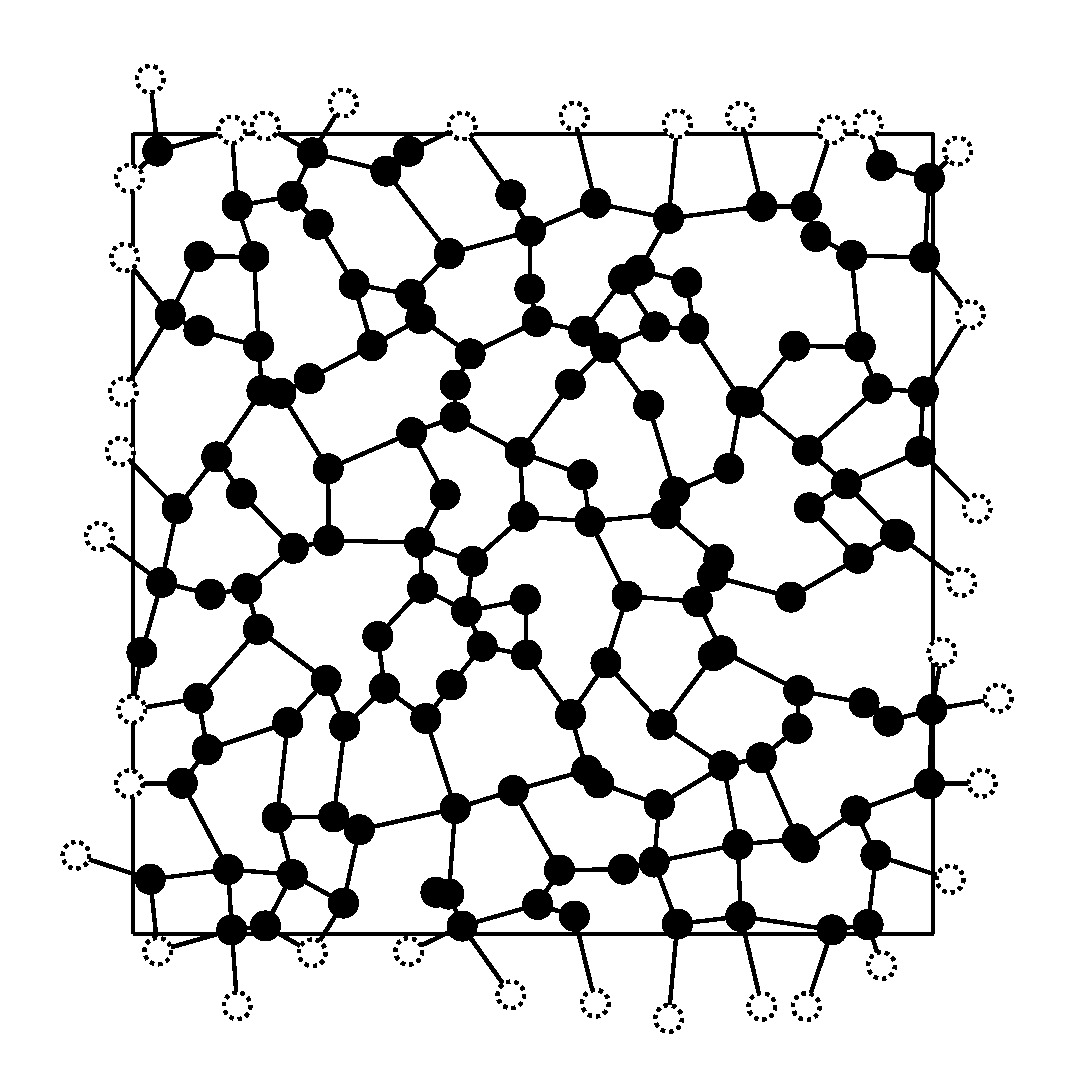
\includegraphics[width=0.14\textwidth]{images/RNG/L12S03.pdf}
        }
        \subfigure[GG example][]{
            \label{sfig:lunes:gg}
            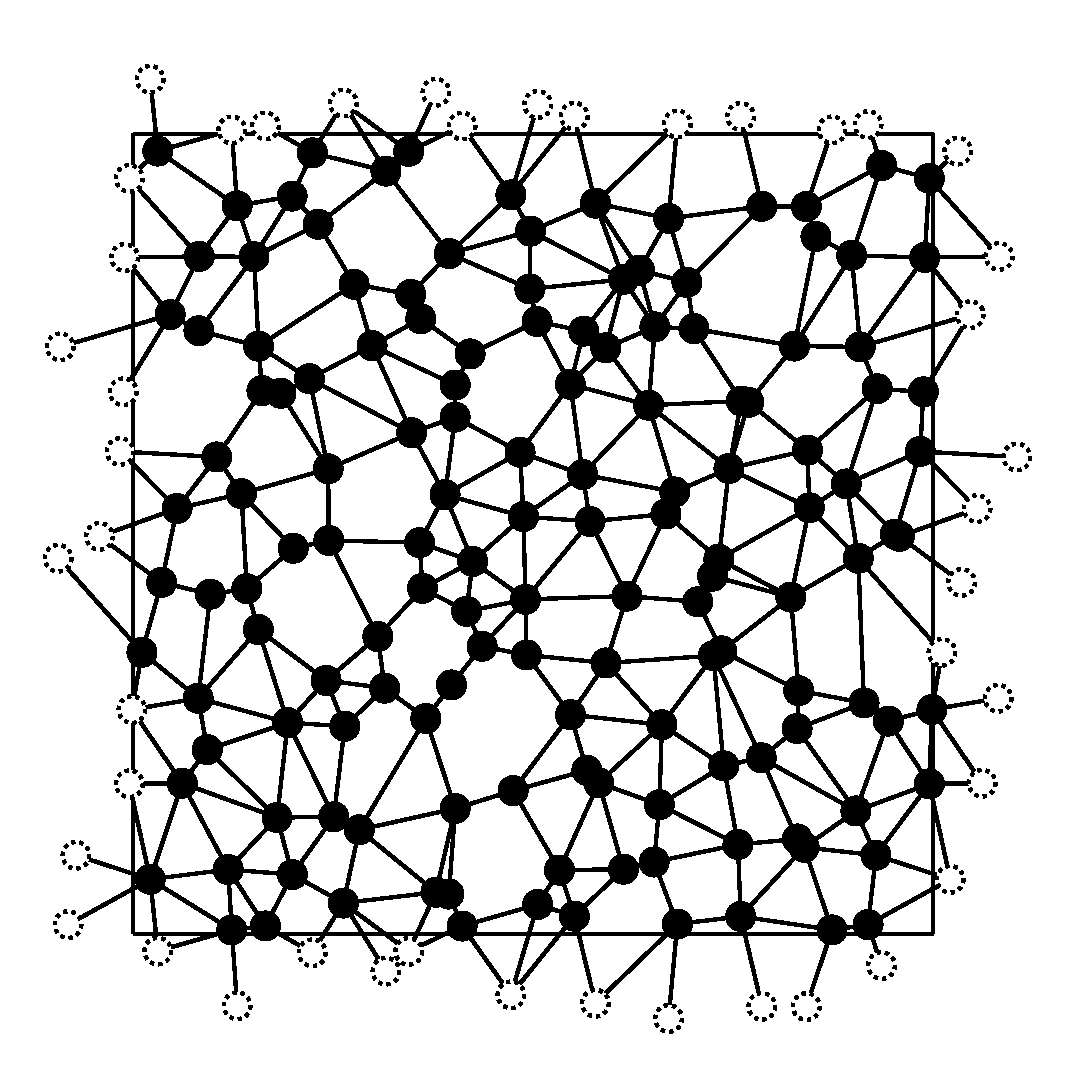
\includegraphics[width=0.14\textwidth]{images/GG/L12S03.pdf}
        }
        \caption[Gabriel - and Relative Neighborhood Graph]
        {
            \subref{sfig:lunes:def} Lunes, which define whether an edge
                exist, of RNG (hatched region) and GG (cross hatched region).
                It is evident from this sketch that the GG is a supergraph
                of the RNG. If there is an edge in the RNG, the hatched
                region contains no node, then of course also the double
                hatched region contains no node and thus this edge appears
                also in the GG. So every egde of the RNG is also present
                in a GG on the same set of nodes.
            \subref{sfig:lunes:rng} Example of a RNG on periodic
                boundary conditions.
            \subref{sfig:lunes:gg} Example of a GG on
                periodic boundary conditions. Periodic nodes are dashed.
        }
        \label{fig:lunes}
    \end{figure}

    % TODO: alles hierdrunter
    \subsubsection{Construction}
        The simplest way to construct these graphs is to test for each
        pair of nodes if any other node lies in
        the lune of the pair. That is of complexity \(O (N^3)\), because
        there are \(N(N-1)\) pairs and for each \((N-2)\) nodes to test. So
        the running time of a straight forward implementation would be of
        order \(O(N^3)\).\\
        To reduce the complexity one can first create a DT in complexity \(O (N \log N)\)
        \cite{RNGCell} and test the connectedness for each edge contained
        therein in \(O (N)\), because the DT is a supergraph of both.
        This results in a complexity of \(O (N^2 \log N)\)
        For the construction of the DT for a given set of points one might
        use existing software libraries, e.g.\ the \texttt{qHull}\cite{qhull} library.\\
        So a trade off is to use basically the simple method but only test
        the connectedness for nodes which are near to the lune and abort if
        one node inside the lune is found. To determine which nodes are
        near the lune one can subdivide the area in \(M\) \emph{cells} of size
        \(L_c \times L_c\) and save for each cell a list with nodes lying
        inside like presented in Ref.\ \cite{RNGCell} and sketched in Fig.\ \ref{fig:cell}.
        The implementation of this thesis uses \(M = N\) (\(L_c = 1\)).
        \begin{figure}[htbp]
            \centering
            %~ 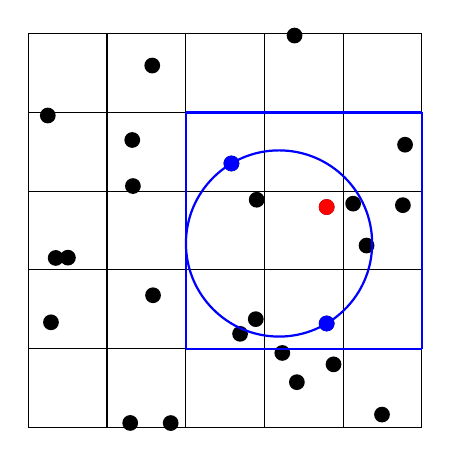
\begin{tikzpicture}
    \foreach \x in {0,1,...,5}{
        \draw (0,\x) -- (5,\x);
        \draw (\x,0) -- (\x,5);
    }
    %random numbers generated by Python
    \foreach \x / \y in {0.28897762565/1.33479488842, 1.29507843519/0.0567389232558, 1.32094528703/3.65045643132, 2.90131976409/2.89143039453, 3.38227004393/4.97678250754, 4.78587153595/3.59043085053, 4.49289684902/0.16312339617, 2.88976245038/1.37508072608, 0.503908610931/2.15612491084, 4.29648323686/2.30979809325, 1.57506933975/4.5958939884, 3.41193951077/0.574638720997, 1.58494426782/1.67834825887, 3.87742721851/0.800878920581, 0.34861369265/2.15217676901, 3.78999774171/1.31996000053, 3.22671310651/0.945568165194, 2.58060642147/3.3521091272, 1.8091306587/0.055518765505, 4.12621981945/2.84187520295, 2.69064049175/1.18843544815, 0.248568008024/3.96126629448, 1.32959523341/3.0654517407, 4.7582022563/2.8223407318, 3.78979061396/2.79890572216}{
        \fill (\x, \y) circle(0.1);
    }
    %~ 2.58060642147/3.3521091272
    %~ 3.78999774171/1.31996000053
    \def\xa{2.58060642147}
    \def\ya{3.3521091272}
    \def\xb{3.78999774171}
    \def\yb{1.31996000053}
    \def\x{3.1853020815900002}
    \def\y{2.3360345638649997}
    \def\d{1.1823977163477497}
    \fill[blue] (\xa,\ya) circle(0.1);
    \fill[blue] (\xb,\yb) circle(0.1);
    \fill[red] (3.78979061396,2.79890572216) circle(0.1);
    \draw[blue,thick] (2,1) -- (5,1);
    \draw[blue,thick] (2,4) -- (5,4);
    \draw[blue,thick] (2,1) -- (2,4);
    \draw[blue,thick] (5,1) -- (5,4);
    \draw[blue,thick] (\x, \y) circle(\d);
\end{tikzpicture}

            %~ 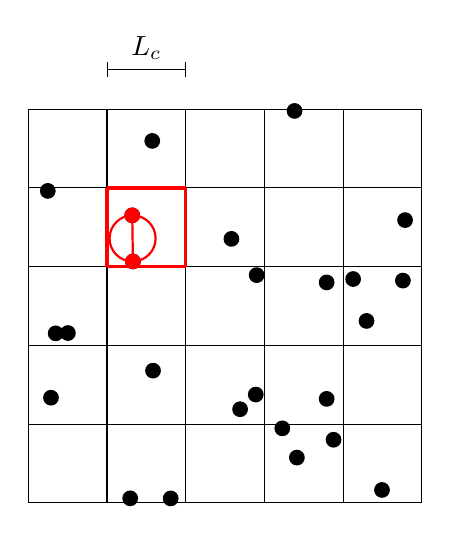
\begin{tikzpicture}
    \draw[|-|] (1,5.5) -- node[above] {$L_c$} (2,5.5);
    \foreach \x in {0,1,...,5}{
        \draw (0,\x) -- (5,\x);
        \draw (\x,0) -- (\x,5);
    }
    %random numbers generated by Python
    \foreach \x / \y in {0.28897762565/1.33479488842, 1.29507843519/0.0567389232558, 1.32094528703/3.65045643132, 2.90131976409/2.89143039453, 3.38227004393/4.97678250754, 4.78587153595/3.59043085053, 4.49289684902/0.16312339617, 2.88976245038/1.37508072608, 0.503908610931/2.15612491084, 4.29648323686/2.30979809325, 1.57506933975/4.5958939884, 3.41193951077/0.574638720997, 1.58494426782/1.67834825887, 3.87742721851/0.800878920581, 0.34861369265/2.15217676901, 3.78999774171/1.31996000053, 3.22671310651/0.945568165194, 2.58060642147/3.3521091272, 1.8091306587/0.055518765505, 4.12621981945/2.84187520295, 2.69064049175/1.18843544815, 0.248568008024/3.96126629448, 1.32959523341/3.0654517407, 4.7582022563/2.8223407318, 3.78979061396/2.79890572216}{
        \fill (\x, \y) circle(0.1);
    }
    %~ 1.32094528703/3.65045643132
    %~ 1.32959523341/3.0654517407
    \def\xa{1.32094528703}
    \def\ya{3.65045643132}
    \def\xb{1.32959523341}
    \def\yb{3.0654517407}
    \def\x{1.3252702602199999}
    \def\y{3.3579540860099999}
    \def\d{0.29253431833708793}
    \fill[red] (\xa,\ya) circle(0.1);
    \fill[red] (\xb,\yb) circle(0.1);
    \draw[red,very thick] (1,3) -- (2,3);
    \draw[red,very thick] (1,4) -- (2,4);
    \draw[red,very thick] (1,3) -- (1,4);
    \draw[red,very thick] (2,3) -- (2,4);
    \draw[red,thick] (\x, \y) circle(\d);
    \draw[red,thick] (\xa, \ya) -- (\xb, \yb) ;
\end{tikzpicture}

            \caption[Sketch how the Cell Method works]
            {
                Sketch how the cell algorithm for the construction of the
                RNG and GG works. Here with the lune definition of the GG.
                The bounding box of the lune, which determines which cells have
                to be tested, is marked with thick colored lines.
                Left: shows that it is sufficient to find a
                single node in an inner cell of the bounding box to discard
                the edge between two distant nodes. The nodes inside the
                other 8 marked cells do not have to be tested anymore.
                Right: shows that only the nodes inside the
                marked cell have to be tested, because there are no other nodes,
                the edge can be drawn.
            }
            \label{fig:cell}
        \end{figure}\\
        Given the discretized cell structure it is just necessary to test the nodes in the cells which
        resemble a rectangular bounding box of the lune. Most pairs will be
        far away from each other and there will be one or more cells in the
        middle of the bounding box, which are completely inside the lune.
        Then only one node has to be tested from such a cell to discard an
        edge between the nodes. On the other hand, nodes that will be connected
        are near to each other so that only very few cells intersect the bounding
        box of their lune and consequently only very few nodes have to be tested.\\
        %~ Here the number of cells equals the number of nodes.
        The complexity of this method should be between \(O(N^2)\) in the
        best case, because for every pair at least one check has to be performed,
        and \(O(N^3)\) in the worst case, e.g.\ all nodes are inside one
        cell.\\
        Combining both algorithms yields a blazing fast algorithm in complexity
        \(O(N \log N)\) for nodes which are evenly spread across the cells.\\
        However, generation of the graphs is not time critical, because
        the MC simulations take much longer. So only the cell algorithm
        was used to gegnerate the graphs.\\
